\chapter[PDF Plots From Matlab]{Bragg Gratings}
\label{AppendixA}
% Tip 4: Example (above) of how to get a shorter chapter title for the Table of Contents 
%======================================================================
\section{Derivation of the 1D Propagation Matrix }
\begin{figure}[h!]
	\centering
	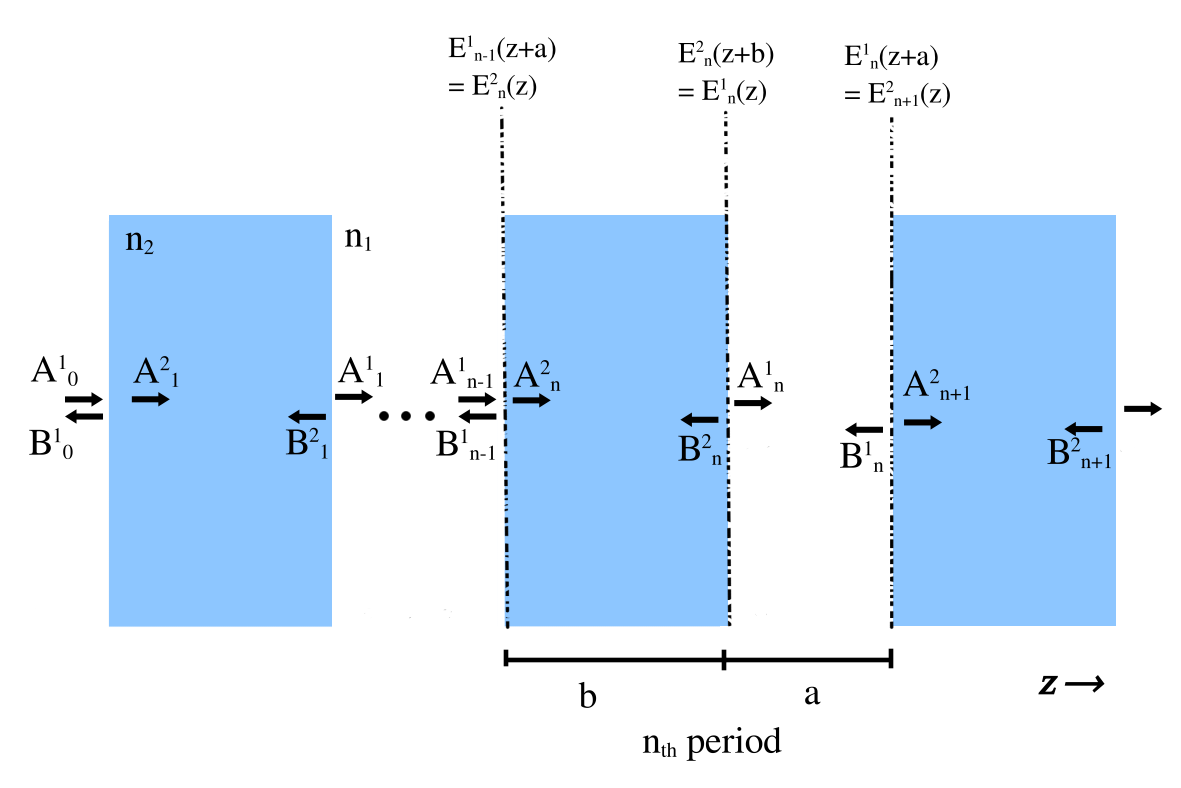
\includegraphics[width=0.7\textwidth]{./Figures/HCPCF/DBR.png}
	\caption{Schematic of quarter wavelength stack}
	\label{1dstack}
\end{figure}

\begin{equation}
	\begin{aligned}
		E^1_n(z) &= A^1_n e^{-ik_{z1}(z-(n-1)a)} + B^1_n e^{ik_{z1}(z-(n-1)a)};  (n-1)a+b<z<na\\
		E^2_n(z) &= A^2_n e^{-ik_{z2}(z-(n-1)a)} + B^2_n e^{ik_{z2}(z-(n-1)a)};  (n-1)a<z<(n-1)a+b\\
	\end{aligned}
\end{equation}
Where $k _j= \frac{2\pi}{n_j}$
The boundary conditions:\\
continuous between the layers:
\begin{equation}
	E^1_n(z) = E^2_n(z+b)
\end{equation}
The second condition is that the electric field is smooth, which can be established in the perpendicular magnetic field. 
i.e. Maxwell's equations for a monochromatic field with freq $\omega$ and time dependence $e^-i\omega t$
\begin{equation}
	\begin{aligned}
		\vec{\nabla}\times\vec{H} &= -i\omega\epsilon(\vec{r})\vec{E}\\
		\vec{\nabla}\times\vec{E} &= i\omega\mu_0\vec{H}	
	\end{aligned}
	\label{eqn:maxwell}
\end{equation}
Assuming that the electric field is linearly polarized $E(z) = \boldsymbol{\hat{x}}E(z)$, then the magnetic field (via Faraday's law) $H(z) = \boldsymbol{\hat{y}}H(z)$ gives the corresponding magnetic field for the two layers 
\begin{equation}
	\begin{aligned}
		H^1_n(z) &=\frac{1}{\eta_1}[A^1_n e^{-ik_{z1}(z-(n-1)a)} - B^1_n e^{ik_{z1}(z-(n-1)a)}]\\
		H^2_n(z) &= \frac{1}{\eta_2}[A^2_n e^{-ik_{z2}(z-(n-1)a)} - B^2_n e^{ik_{z2}(z-(n-1)a)}]
	\end{aligned}
\end{equation}

\begin{equation}
	\begin{aligned}
		A^2_n(z) = \frac{1}{2}[E^2_n(z) + \eta_2 H^2_n(z)]\\
		B^2_n(z) = \frac{1}{2}[E^2_n(z) - \eta_2 H^2_n(z)]
	\end{aligned}
\end{equation}
Where the impedance $\eta_2 = \frac{\eta_0}{n2}$ \\
Putting these relations into a matrix form we can find a a solution for the transition boundary:
\begin{equation*}
	\begin{aligned}
		\begin{bmatrix}E^1_{n-1}(z+a)\\H^1_{n-1}(z+a) \end{bmatrix} 
		&= \begin{bmatrix}E^2_n(z)\\H^2_n(z) \end{bmatrix}\\
		\begin{bmatrix}1 & 1\\\eta_1^{-1} & -\eta_1^{-1}\end{bmatrix}\begin{bmatrix}A^1_{n-1}(z+a)\\B^1_{n-1}(z+a) \end{bmatrix}
		&=\begin{bmatrix}1 & 1\\\eta_2^{-1} & -\eta_2^{-1}\end{bmatrix}\begin{bmatrix}A^2_n(z)\\B^2_n(z) \end{bmatrix} \\
		\begin{bmatrix}A^1_{n-1}(z+a)\\B^1_{n-1}(z+a) \end{bmatrix}
		&= M_{1\rightarrow2}\begin{bmatrix}A^2_n(z)\\B^2_n(z) \end{bmatrix}\\
	\end{aligned}
\end{equation*}

\begin{equation}
	\begin{bmatrix}A^1_{n-1}(z+a)\\B^1_{n-1}(z+a) \end{bmatrix}
	= M_{1\rightarrow2}\begin{bmatrix}A^2_n(z)\\B^2_n(z) \end{bmatrix}\\
\end{equation}

The transition matrix:
\begin{equation}
	M_{1\rightarrow2} = 
	\frac{1}{2}\begin{bmatrix}1+\frac{k_2}{k_1} & 1-\frac{k_2}{k_1}\\1-\frac{k_2}{k_1} & 1+\frac{k_2}{k_1}\end{bmatrix}
\end{equation}

The plane wave propagating though the material will acquire a phase:  
\begin{equation}
	M_{n_2} = \begin{bmatrix}e^{ik_{z2}b} & 0\\0 & e^{-ik_{z2}b}\end{bmatrix}\\
\end{equation}

Thus the travel through the n2 material can be summarized by
\begin{equation}
	\begin{aligned}
		\begin{bmatrix}A^1_{n-1}(z+a)\\B^1_{n-1}(z+a) \end{bmatrix}
		M_{1\rightarrow2}M_{n2}
		\begin{bmatrix}A^2_n(z+b)\\B^2_n(z+b) \end{bmatrix}
	\end{aligned}
\end{equation}

For the electric field through the n1 region :
\begin{equation}
	M_{1\rightarrow2} = 
	\frac{1}{2}\begin{bmatrix}
		1+\frac{k_1}{k_2} & 1-\frac{k_1}{k_2}\\
		1-\frac{k_1}{k_2} & 1+\frac{k_1}{k_2}
	\end{bmatrix}
	\begin{aligned}
		&M_{n_1} =
		\begin{bmatrix}
			e^{ik_{z1}a} & 0\\
			0 & e^{-ik_{z1}a}
		\end{bmatrix}\\
	\end{aligned}
\end{equation}

Becomes one periodic transition matrix:
\begin{equation*}
	M_p = M_{1\rightarrow2}M_{n2}M_{2\rightarrow1}M_{n1} = \begin{bmatrix}m_{11} & m_{12}\\m_{21} & m_{22}\end{bmatrix}\\ 	
\end{equation*}

For an N period block:
\begin{equation}
	\begin{aligned}
		\begin{bmatrix}A_0\\B_0 \end{bmatrix} 
		&=(M_p)^N 
		\begin{bmatrix}A_{(N+1)}\\0\end{bmatrix}\\
	\end{aligned}
\end{equation}
